%\documentclass[sigconf, review, anonymous, screen]{acmart}
\documentclass[sigconf, screen]{acmart}
% The preceding line is only needed to identify funding in the first footnote. If that is unneeded, please comment it out.
\usepackage{kotex}
\usepackage{amsmath,amssymb,amsfonts}
\usepackage{algorithmic}
\usepackage{graphicx}
\usepackage{textcomp}
\usepackage{xcolor}
\usepackage{balance}

\usepackage[ruled,vlined,linesnumbered]{algorithm2e}

\usepackage{booktabs} % For formal tables
\usepackage{subcaption} % for subfigures

\usepackage{fancyhdr}
\usepackage{tabularx}
\usepackage{multirow}
\usepackage{multicol}
\usepackage{mdwlist}
\usepackage{indentfirst}
\usepackage{physics}
\usepackage{xspace}
\usepackage{tablefootnote}
%\usepackage[bottom]{footmisc}
%\usepackage{footnote}
\usepackage{hyperref}
\usepackage{makecell}
\usepackage{subcaption}
\usepackage[bottom]{footmisc}
\usepackage{balance}
\xspaceaddexceptions{]\}}

\setcopyright{none}
\renewcommand\footnotetextcopyrightpermission[1]{}
\settopmatter{printacmref=false}


%\acmConference[KDD'19]{ACM SIGKDD Conference}{Aug 2019}{Anchorage, Alaska USA}
\acmConference[]{}{}{}
\acmYear{2019}
\copyrightyear{2019}

% Definitions
\newcommand{\blue}[1]{{\color{blue} #1}}
\newcommand{\red}[1]{{\color{red} #1}}
\newcommand{\orange}[1]{{\color{orange} #1}}

% math symbol definitions
\newcommand{\mat}[1]{\mathbf{#1}}
\newcommand{\ve}[1]{\mathbf{#1}}
\newcommand{\set}[1]{\mathbb{#1}}
\newcommand{\seq}[2]{\mathcal{#1}^{#2}}

% paper-dependent definitions
\newcommand{\User}{\set{U}}
\newcommand{\Item}{\set{I}}
\newcommand{\Su}{\seq{S}{u}}

% pre-defined names
\newcommand{\dqnname}{\textsc{DQN}}
\newcommand{\dqn}{\dqnname\space}

\newcommand{\sdqnname}{\textsc{S-DQN}}
\newcommand{\sdqn}{\sdqnname\space}

\newcommand{\sadqnname}{\textsc{SA-DQN}}
\newcommand{\sadqn}{\sadqnname\space}

\newcommand{\sapdqnname}{\textsc{SA-DQN+}}
\newcommand{\sapdqn}{\sapdqnname\space}


%\setlength{\belowcaptionskip}{-0.3cm}

\begin{document}
\title[Super Mario RL]{대규모 데이터분석 특강 - 프로젝트 제안서}

\author{구본헌}
\affiliation{
  \institution{컴퓨터 공학부}
  \institution{서울대학교}
}
\email{darkgs@snu.ac.kr}

\author{김정훈}
\affiliation{
  \institution{컴퓨터 공학부}
  \institution{서울대학교}
}
\email{rlawjdgns434@snu.ac.kr}

% Sec 0. Abstract
\begin{abstract}
	블라블라~\ref{DQN}
\end{abstract}

%\keywords{
%Reinforcement Learning; 강화 학습
%}

\maketitle
% Sec 1. Introduction
\section{Introduction}
\label{sec:intro}
본 대규모 데이터분석 특강 프로젝트에서 우리는 슈퍼 마리오 브라더스 게임을 강화학습을통해 컴퓨터가 학습하고 최종적으로 높은 점수로 스테이지를 클리어 하는 것을 목표로 한다.

슈퍼 마리오 브라더스에서 사용 가능한 동작은 총 6 가지로 구성되어 있으나 서로 다른 키를 조합하여 입력하는 것이 가능하므로 실제로 사용 가능한 동작은 총 16개로 구성되어 있다. 해당 게임은 agent인 마리오가 목적지에 도달하거나, 적에게 부딪히거나, 제한 시간 내에 목적지에 도달하지 못하면 stage가 끝남으로써 episodic한 요소를 가지고 있다. 

따라서 해당 게임을 강화학습을 통해 클리어하기 위해 실제 인간에게 주어지는 것처럼 현재 화면을 입력 값으로 받고 이를 통해 최적의 동작(action)을 찾아내는 모델인 convolutional neural network (CNN)을 구축하는 것을 기반으로 다양한 시도를 할 것이다.

프로젝트 기간내에 효율적으로 시간을 분배해 최적의 결과를 도출하기 위해 각 구성원의 역할을 개발환경 세팅, 기존 방법 학습, 새로운 방법 연구, 제안 방법 개발과 같은 방식으로 세분화한다.

해당 프로젝트 제안서의 구성은 다음과 같다. 
2 장에서는 본 프로젝트에서 풀려고 하는 슈퍼 마리오 브라더스 게임을 학습하고 목표를 달성하기 위해 도움이 될만한 기존 논문의 메인 아이디어를 간략히 설명하고 어떻게 프로젝트 구현에 사용될 수 있을지에 대해 설명한다. 
또한 논문의 메소드를 본 프로젝트에서 사용함에 있어 제약사항 혹은 문제가 될 여지가 있다면 이러한 부분에 대해 서술한다. 
3 장에서는 슈퍼 마리오 브라더스 게임에 대해 간략히 설명하고 강화학습을 진행하는데 필요한 state, action, 그리고 reward이 게임에서 어떻게 구성되어 있는지에 대해 설명한다. 
4 장에서는 본 프로젝트에서 사용할 라이브러리에 대한 설명과 각 구성원의 개발 일정에 따른 역할에 대해 설명한다. 
마지막으로 5 장에서는 해당 제안서에서 설명한 부분들에 대해 정리한 뒤 본 프로젝트 제안서를 마무리하는 것으로 구성되어 있다.

\section{Survey}
\label{sec:survey}
\subsection{Playing Atari with Deep Reinforcement Learning}
\label{sec:survey:DQN}
해당 논문~\cite{DQN}은 딥러닝 알고리즘으로 action-value function의 Q 값을 예측하는 기법인 Deep Q-Networks (DQN)을 제시하였다. 
논문 제목에서도 볼 수 있듯이 새로운 메소드를 Atari 2600이라는 고전 게임 모음 중 대표적인 7 개의 게임을 통해 그 성능을 확인하였다. 
Atari 2600 게임은 action에 대한 transition 확률과 reward가 명시적으로 주어지지 않은 model-free 문제이다.

해당 논문에서 볼 수 있는 특이한 점은 입력 값으로 게임의 이미지 전체를 받는다는 점인데, 기존 강화 학습에서 state를 정의할 때 게임 이미지의 각 픽셀을 하나의 state로 정의하여 에이전트에게 전달하는 것과는 다르면서 색다른 방식이다. 
따라서 게임의 이미지 화면을 입력 값으로 받으면 딥러닝 알고리즘에서 이미지 처리에 탁월한 Convolutional Neural Networks (CNN)을 통해 계산된 Q값을 에이전트에게 전달하고 해당 값을 기반으로 최적의 action을 실행하여 게임을 진행하는 방식으로 구성되어 있다. 

여기서 눈 여겨 봐야할 점은 Q값을 구하기 위해 CNN을 사용하였다는 것인데, 이는 기본적으로 사용되는 value iteration 알고리즘과 같은 문제점을 해결한다. 
Value iteration 알고리즘은 논문과 같은 환경인 transition 확률과 reward가 명시적으로 주어지지 않은 조건에서는 동작하기 어려운 점이 있다. 
그러나 해당 논문에서 사용하는 Q-Networks는 이러한 model-free 문제에서 neural network value function approximator를 통한 샘플링을 통해 Q값을 구한다. 
따라서 학습을 할 때 Q-network에서는 손실 함수를 최소화하면서 그 성능을 높인다. 

논문에서 보여준 이러한 방식은 우리가 풀려는 슈퍼마리오 게임에서의 환경과 비슷한 점이 많기 때문에 논문에서 제시한 DQN 알고리즘을 사용할 예정이다. 
슈퍼마리오 게임 또한 Atari 게임과 같이 게임 화면이 state로 주어지고 finite한 게임 내에서 게임이 한 에피소드를 끝내기 위한 조건도 유사하기 때문에 논문에서 제시한 알고리즘을 사용한다면 높은 성능을 보일 것이라 판단한다. 

그러나 해당 논문에서 제시한 DQN은 Q-learning 값을 업데이트 하는 과정에 있어서 max 연산자를 사용하기 때문에 Q-value를 실제보다 높게 평가하고 그 결과 학습이 느려지는 경향이 있다. 
따라서 실험에 사용한 Atari 게임은 우리가 풀려는 슈퍼마리오 게임보다 상대적으로 크기가 작고 간단하기 때문에 슈퍼마리오 게임과 같이 더 크고 복잡한 조건에서도 과연 학습이 느려질 수 있다는 것에 대한 제약사항이 존재할 가능성이 있다. 


\subsection{Dueling Network Architectures for Deep Reinforcement Learning}
DQN알고리즘이 큰 성과를 이루며 deep Q learning에 대한 발전 속도는 굉장히 빨라졌는데, 해당 논문 또한 DQN 알고리즘을 기반한 새로운 네트워크 구조를 개발한 논문이다. 
기존의 DQN은 특정 지점에서의 Q function을 추정(estimate)하기 위하여 모든 state와 action의 값을 모두 평가해야 한다. 
그러나 대부분의 경우에는 state의 가치가 중요하고 action으로 인한 가치의 변화가 극명한 경우는 많지 않다. 
따라서 해당 논문은 Figure~\ref{fig:dueling_network}과 같이 새로운 DQN 구조(dueling network)를 제안했다.

\begin{figure}[h]
\begin{center}
\begin{tabular}{c}
     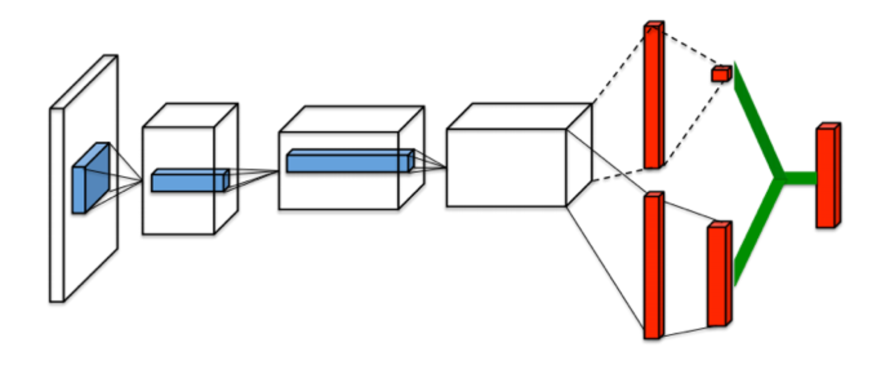
\includegraphics[width=0.45\textwidth]{FIG/DuelingNetwork.png} \\
\end{tabular}
\caption{
	Dueling Network의 구조.
}
\label{fig:dueling_network}
\end{center}
\end{figure}

앞서 말한 것처럼, 해당 논문에서의 네트워크 구조는 새로운 DQN 구조를 가지고 있는데 Q 값의 정의로부터 유도되는 한 가지 수식에서 아이디어를 얻어 탄생했다. 
해당 수식은 아래와 같다. 
\begin{align*}
	Q(s,a) = V(s) + A(s,a) \\
\end{align*}
Q 값의 의미는 현재 상태에서 행동을 취할 때 얻을 수 있는 보상의 합을 말한다. 
해당 논문에서는 이 값을 두가지로 분리하였는데 Value function(V)와 Advantage function(A)이다. 
V 값은 현재 상태에서 최선의 행동을 취했을 때 얻을 수 있는 보상의 합이고, A는 최선인 행동과 다른 행동들 사이의 보상의 차를 의미한다. 
이러한 구조를 자세히 보면 Q 값을 추론하는 것을 두 가지로 분리해서 생각한 것인데, 현재 상태가 좋은지 나쁜지를 V 값으로 추론하고 그 중에서 어떤 행동을 고를지를 A 값을 이용하여 추론한다. 
따라서 V 값은 바이어스 같은 역할을 하고 V를 중심으로 좋고 나쁨을 A 값을 이용하여 추론하게 되는 것이다. 

Dueling Network 또한 DQN과 마찬가지로 게임 이미지를 입력 값으로 받아 Q 값을 추정(estimate)한다. 
해당 논문에서 제시한 알고리즘은 Atari 게임에서 DQN을 더불어 다른 메소드보다 높은 성능을 보였다.

앞서 말한 것과 같이 우리의 프로젝트 또한 Atari 게임과 비슷한 환경을 가지고 있기 때문에 해당 알고리즘을 사용하여 성능을 높일 수 있을 거라 판단한다. 
또한 논문에서는 해당 알고리즘은 기존에 존재하는 여러 알고리즘(DQN, SARSA)에서도 사용될 수 있다고 설명한다. 
따라서 프로젝트에서 DQN으로 시도를 할 것을 염두하고 있기 때문에 DQN 혹은 DDQN을 사용할 경우 해당 알고리즘을 추가하여 손쉽게 성능을 높이기 위한 추가적인 시도를 할 것이다.

\subsection{Deterministic Policy Gradient Algorithms}
\label{sec:survey:DPG}
앞서 살펴본 DQN과 같은 방법은 value function을 학습하는 방식이기 때문에 만약 value가 살짝 바뀌어도 policy가 같이 변하여 학습 과정이 불안정하게 되고 수렴이 불안정해지는 단점이 있다. 
따라서 policy 자체를 예측을 하면 되지 않을까라는 개념으로 탄생한 것이 policy gradient 알고리즘이다. 

policy gradient 알고리즘은 expected reward를 policy의 파라미터에 대한 함수로 모델링하고 이 reward를 최대화하는 policy를 gradient ascent 기법을 사용해서 찾는 기법이다.
해당 기법은 policy의 변화를 통해 더 나은 policy를 찾아가는 방식으로 구성되어 있다. 
최적의 policy는 stochastic한 성질을 가지는 경우가 많기 때문에 stochastic policy gradient 방식을 선호하였는데 해당 논문을 통해 deterministic policy gradient가 high-dimensional task에서 보다 빠르게 동작한다는 것을 증명하였다. 

해당 논문에서는 octopus arm 실험을 통해 성능을 측정하였는데 해당 실험을 사용한 이유는 high dimensional task에서의 성능을 확인하기 위함이다 (Figure~\ref{fig:dueling_network} 참조).
해당 실험에서 목표는 6 개의 구획으로 구성된 다리를 움직여 오렌지 색상의 음식을 검은색 입으로 전달하여 보상을 얻는 것이다.
환경에서는 50 개의 continuous 한 state가 존재하며 각 구획에는 회전 및 이동할 수 있는 muscle이 존재해 한 구획당 총 20 가지의 동작이 가능하다. 
이러한 실험에서 높은 성능을 보였고 high dimensional 한 task에서는 deterministic policy gradient 알고리즘이 stochastic의 경우보다 성능이 좋다는 것을 확인하였다.

\begin{figure}[h]
\begin{center}
\begin{tabular}{c}
     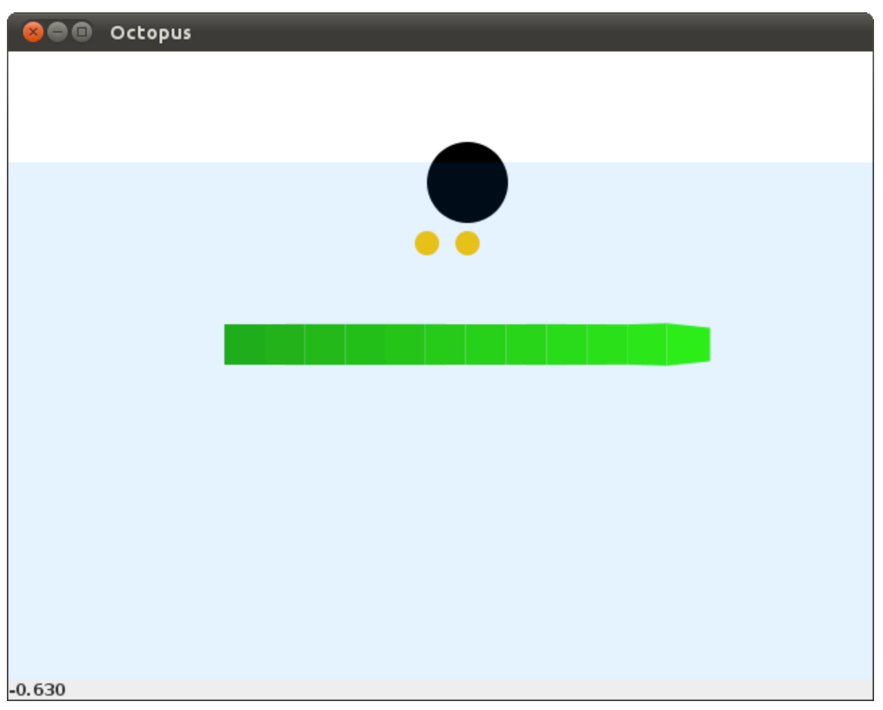
\includegraphics[width=0.45\textwidth]{FIG/OctopusArm.png} \\
\end{tabular}
\caption{
	Octopus Arm Environment.
}
\label{fig:octopus_arm}
\end{center}
\end{figure}

policy gradient 알고리즘은 continuous 한 action space 상황에서 자주 사용되는데 본 프로젝트에서 실험하는 슈퍼 마리오 브라더스는 discrete 한 action space 상황이기 때문에 deterministic policy gradient 알고리즘을 바로 적용할 수는 없다. 
그러나 해당 논문을 통해 우리 모델의 성능을 높이기 위해 policy gradient를 적용한다는 아이디어를 참고할 수 있기에 해당 논문을 서베이 목록에 추가하였다.

\subsection{Deep Deterministic Policy Gradient}
Deep Deterministic Policy Gradient (DDPG)는 state와 action을 입력으로 받아 각 action에 대한 value값을 산출해내는 Q-function을 학습시키는 방법이다.
DDPG의 핵심 동작은 아래와 같은 식으로 나타낼 수 있다.
\begin{align*}
	a^*(s) &= arg \underset{a}{max} Q^*(s,a) \\
\end{align*}
%\begin{align*}
%	h_t &= f(h_{t-1},x_t;W,b) \\
%		&= \tanh{(W_{hh}h_{t-1}+W_{hx}x_t+b_h)} \\
%		&= \tanh{(W_{h}[h_{t-1},x_t]+b_h)}
%\end{align*}
여기서 Q-function Q 는 action a와 state s를 입력으로 받아 value를 판별해주므로 최대 value를 가지는 action을 선택하면 최적화된 policy를 구할 수 있다.

DDPG는 다음과 같은 특징을 가지고 있다.
\begin{itemize}
	\item off-policy 방법
	\item continuous action space에서만 동작하는 방법
	\item 병렬화된 학습 방법을 제공하지 않음
\end{itemize}
본 프로젝트에서 학습하기로 한 게임인 슈퍼 마리오 브라더스는 discrete한 action space를 가지므로 DDPG 알고리즘을 바로 적용할 수는 없다.
하지만 DDPG에서 학습을 돕기 위한 주요 아이디어를 차용하여 우리 프로젝트에 적용해 볼 수 있다.

\paragraph{\textbf{Replay Buffer:}}
음냐
\paragraph{\textbf{Target Network:}}
음냐

\subsection{Asynchronous Actor-Critic}
Volodymyr Mnih, et. al. 이 제안한 Asynchronous Actor-Critic (A3C)~\cite{A3C}는 게임 플레이를 위한 강화학습에 널리 쓰이는 방법이다.


\subsection{Double Q-learning}
...


\section{Proposed Method}
\label{sec:method}
이번 섹션에서는 슈퍼 마리오 브라더스 

\subsection{Super mario bros}

\begin{figure}[]
\begin{center}
\begin{tabular}{c}
     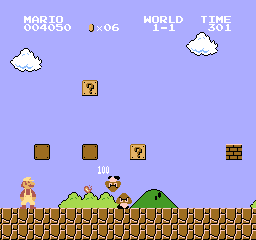
\includegraphics[width=0.45\textwidth]{FIG/SuperMarioBros.png} \\
\end{tabular}
\caption{
	슈퍼 마리오 브라더스의 게임 화면.
}
\label{fig:mario_title}
\end{center}
\end{figure}

슈퍼 마리오 브라더스는 닌텐도 초기의 액션 게임으로 1985년 9월 13일 NES (Nintendo Entertainment System) 전용 게임으로 출시 되었다.
Figure~\ref{fig:mario_title}은 이 게임의 플레이 화면이다.
당시 출시된 다른 게임들과 비교하여 우수한 조작감과 완성도 높은 미술로 크게 흥행하였으며 현재 2019년도 까지고 지속적으로 후속작이 출시되고 있다.
간단한 조작으로도 자유도 높은 플레이가 가능하여 강화학습의 목표로 삼기에 적합하여 이번 프로젝트의 대상으로 선택하였다.
슈퍼 마리오 브라더스는 총 8개의 world 와 각 world 당 4개의 stage로 구성되어 있다.
각 world 별로 특징있는 컨셉을 (물의 나라, 얼음의 나라, 등) 가지고 디자인 되어 배경 및 등장하는 적 케릭터가 차이가 있다.
또한 world 및 stage 수가 증가할 수록 난이도가 올라가는 경향을 가진다.

\begin{table}[]
	\caption {
		슈퍼 마리오 브라더스에서 가능한 키 입력. 서로 다른 키를 조합하여 입력하는 것이 가능하다.
	}
	\label{tab:mario:key}
\begin{tabular}{lr}
\toprule
키     & \multicolumn{1}{c}{동작 설명} \\
\midrule
up    & 특수한 상황(넝쿨, 파이프)에서 마리오를 위로 이동 \\
left  & 마리오를 왼쪽으로 이동 \\
down  & 특수한 상황(넝쿨, 파이프)에서 마리오를 아래로 이동 \\
right & 마리오를 오른쪽으로 이동 \\
A     & 가속 또는 불꽃 공격(슈퍼 마리오만 해당)\\
B     & 점프 \\
\bottomrule
\end{tabular}
\end{table}

Table~\ref{tab:mario:key} 에서 슈퍼 마리오 브라더스 게임에서 가능한 모든 키 입력을 소개한다.
모든 입력은 중복하여 입력하여 마리오가 다른 동작을 하게 할 수 있다.
예를 들면 right 키와 B 키를 동시에 입력하면 마리오가 오른쪽으로 나아가며 점프한다.
하지만 경우에 따라 right 키와 left 키를 동시에 누른 경우 처럼 상보적인 두 가지 키를 조합하는 경우 무의미한 동작을 나타낼 수도 있다.
슈퍼 마리오 브라더스 게임에서 유의미한 키조합을 고려할 경우 가능한 Action의 경우의 수는 16가지 이다.

슈퍼 마리오 브라더스에서 목적지인 깃발로 이동하면 한 stage가 종료된다.
그 외에는 적에게 부딧치거나, 함정에 빠진 경우, 그리고 제한 시간이 지난 경우 stage가 종료되며 처음부터 다시 시작하게 된다.
이 게임의 목적은 보다 많은 점수를 얻으면서 깃발에 도달하여 stage를 완료하는 것이다.
stage 내부에서 점수를 얻는 방법은 아래와 같다.
\begin{itemize}
	\item \textbf{깃발 도달시 남은 시간:}
		제한 시간 이내에 깃발에 도달한 경우 남은 시간 (초 단위)당 100점 획득.
	\item \textbf{동전을 획득:}
		stage내에서 벽돌, 물음표 블록, 그리고 동전 아이템을 통해 동전에 닿으면 100점 획득.
	\item \textbf{버섯, 꽃을 획득:}
		stage내의 물음표 블록에서 버섯 또는 꽃이 나왔을 때 닿으면 100점 획득.
	\item \textbf{적을 처치:}
		적을 처치시 기본적으로 100점 획득하며 연속된 처치를 할 경우 매번 2배의 추가 점수 획득.
\end{itemize}

이 게임에서 stage별로 목적지에 도달하지 못하고 종료된 경우 다시 도전할 기회를 부여하는 데 이 횟수는 마리오의 남은 생명으로 결정된다.
게임내에서 녹색 버섯을 획득하거나 동전을 100개 모은 경우 추가로 보너스 생명을 1개 얻게 된다.
강화학습을 위한 환경에서는 학습을 시키기 위해 stage를 수 많이 반복하여야 하여 이러한 재도전 횟수를 제한하는 것을 해제한 상태에서 학습시키게 된다.
하지만 실제 플레이어가 게임을 한다고 가정할 때 이러한 생명을 관리하는 것은 게임을 끝까지 완수하기 위한 중요한 요소이다.

\subsection{Basis for reinforcement learning}
강화학습에서 현재 state는 이 후 action을 결정하는 데 중요한 요소이다.
실제 게임 플레이어와 공평한 조건에서 경쟁하기 위해 본 프로젝트에서 state를 화면에 표시되는 이미지를 사용하여 결정하기로 하였다.
Convolutaionl neural network (CNN)~\cite{CNN}은 이미지로 부터 학습 모델에 필요한 feature를 추출하여 의사 결정에 활용하는 널리 알려진 방법이다.
본 프로젝트에서 우리는 화면 이미지를 CNN을 통해 해석하여 게임 점수를 최대한 얻을 수 있는 action을 추론하는 모델을 만들고자 한다.

우리는 키 조합을 통해 action을 생성할 수 있는데 유의미한 조합만을 고려하면 아래와 같은 16개의 키조합을 각각의 action으로 정의한다.
\begin{enumerate}
	\item 아무키도 누르지 않음
	\item left
	\item right
	\item up
	\item down
	\item A
	\item B
	\item A + B
	\item left + A
	\item left + B
	\item left + A + B
	\item right + B
	\item right + A
	\item right + A + B
	\item up + B
	\item down + B
\end{enumerate}
우리의 모델은 최종적으로 Figure~\ref{fig:overview}와 같이 현재 state에서 각 차원이 각 action에 대응되는 16차원의 vector를 산출하여 각 action의 적합성을 확률적으로 추론한다.
\begin{figure}[]
\begin{center}
\begin{tabular}{c}
     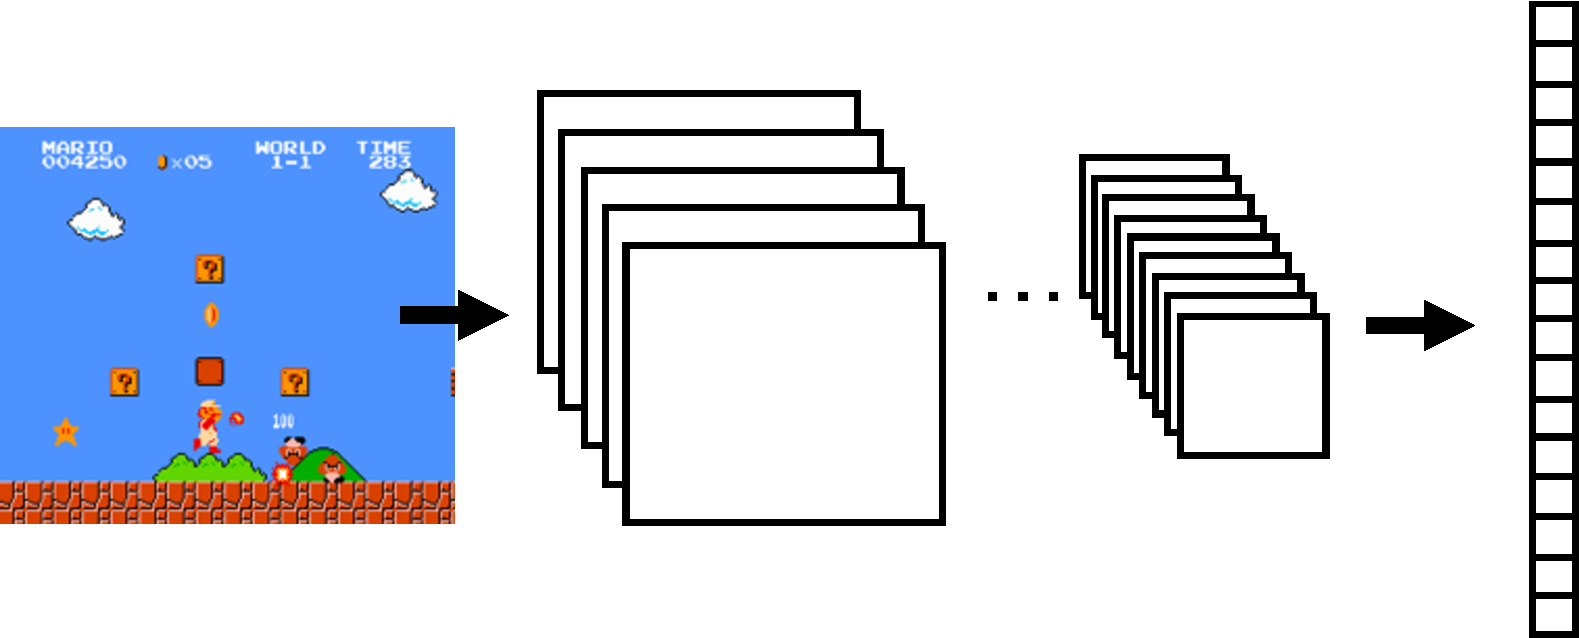
\includegraphics[width=0.45\textwidth]{FIG/overview.pdf} \\
\end{tabular}
\caption{
	게임 화면으로부터 action을 추론하기 위한 모델. CNN을 통해 게임화면을 해석하여 16차원의 action의 적합성을 추론한다.
}
\label{fig:overview}
\end{center}
\end{figure}

강화학습에서 모델은 현재 state에서 최종적으로 얻을 수 있는 reward를 극대화하는 action을 선택하도록 학습된다.
따라서 reward를 잘 설정해야 올바른 선택을 하도록 유도할 수 있다.
슈퍼 마리오 브라더스 게임에서 stage가 끝날 때 남은 시간당 100점을 획득하게 된다.
이는 다른 방법으로 얻는 점수보다 상당히 많은 양이다.
따라서 획득 점수 위주로 reward를 설정하였을 때, 마리오가 빠른 시간안에 깃발로 도달하도록 유도할 수 있다.
또한, stage 중간에 코인, 아이템, 그리고 적을 처치해서 얻는 점수를 고려하면 중간중간의 imediate reward로 활용되어 마리오가 해당 동작을 하도록 하는 학습을 할 수 있다.
이와 같이, stage 내부의 획득 점수를 통해 reward를 주는 것은 올바른 게임 플레이를 학습하는 데 도움을 준다.

게임의 특성상 마리오를 큰 마리오, 나아가 슈퍼 마리오로 변신시키면 남은 stage를 진행함에 있어 크게 유리한 요소로 작용한다.
우리 모델이 슈퍼 마리오로 변신하는 것을 지향하고 변신이 풀리는 것을 지양하기 위해 상위 단계로 변신할 때 획득 점수이외의 부가적인 reward를 할당하고, 변신이 풀릴 경우 reward를 크게 감소시키도록 한다.

\subsection{State from partial area}
사람들이 슈퍼 마리오 브라더스를 실제로 플레이할 때, 사람들은 상황에 따라 화면의 일부분을 좀 더 집중해서 바라보게 된다.
예를 들면, 마리오가 공중에서 하강하고 있을 때는 마리오의 아래 쪽에 집중하여 바닥의 함정을 피하거나 적을 밟아 처치하도록 조작한다.
전반적으로, 전체 화면의 내용보다 마리오 주변에서 일어나고 있는 일에 집중하는 경향이 있다.

\begin{figure}[]
\begin{center}
\begin{tabular}{c}
     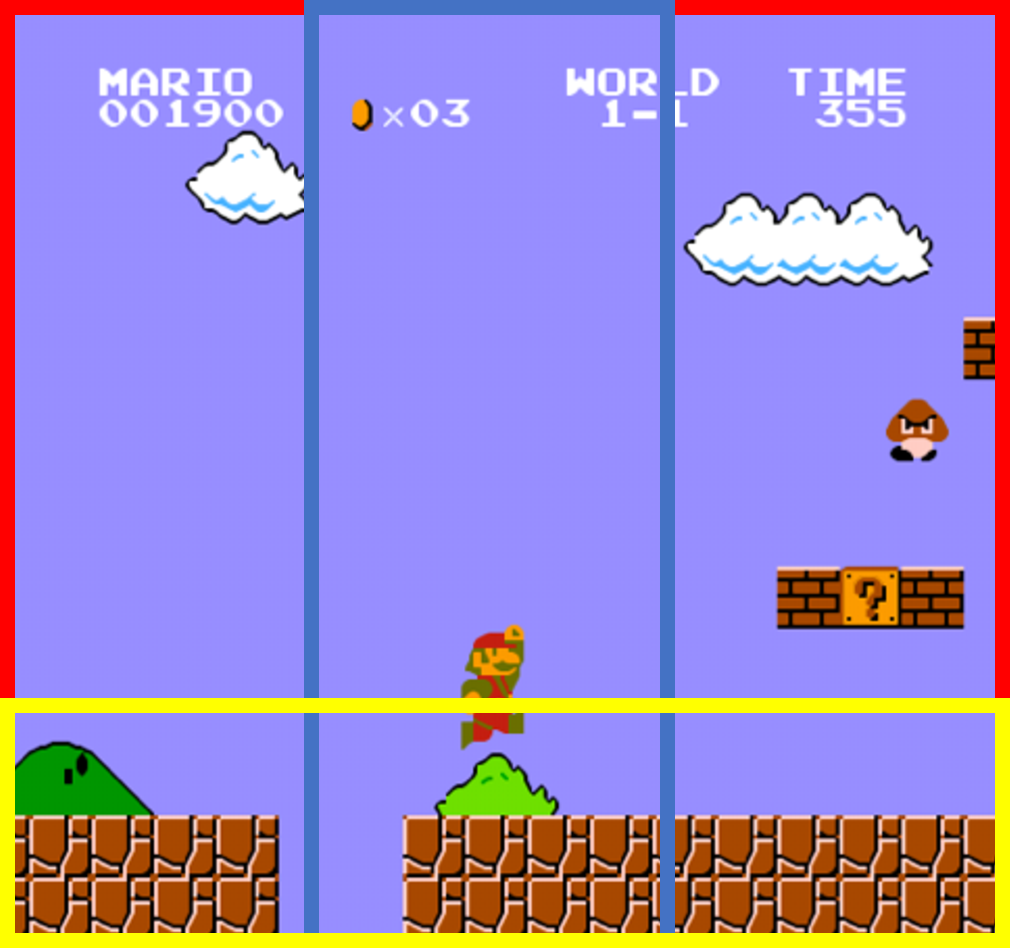
\includegraphics[width=0.4\textwidth]{FIG/split_screen.pdf} \\
\end{tabular}
\caption{
	화면 분할을 통해 여러 CNN 입력을 생성하는 예시. 전체 화면을 나타내는 빨간색, 마리오 주변을 나타내는 파란색, 그리고 바닥의 함정을 조심하기 위한 노란색 영역이 있다.
}
\label{fig:split_screen}
\end{center}
\end{figure}

이러한 게임의 특성을 고려하여 우리 모델도 여러 개의 CNN을 만들어 화면의 각 구역별로 따로 feature를 추출하기로 한다.
이렇게 추출한 feature의 중요도는 마리오의 상황에 따라 변화한다. 앞서 예와 같이 마리오가 공중에 있다면 마리오 주변에 좀 더 집중해야 한다.
만약 마리오의 달리기 속도가 빠른 상황이라면 좀 더 전체 화면부위를 고려하여 다음 action을 정해야한다.
또한 바닥의 함정에 빠지면 마리오가 즉사할 수 있으므로 아래 쪽 영역에 대한 주의도 늦출 수 없다.
우리 모델에서는 figure~\ref{fig:split_screen}과 같이 여러 구역으로 나눠 입력을 만든 후 각각의 CNN으로 생성된 feature를 마리오의 현재 상황에 따라 중요도를 계산하도록 attention layer를 통해 현재 feature를 결정하도록 한다.




\section{Development Plan}
\label{sec:plan}
....


\section{Conclusion}
\label{sec:conclusion}
지금까지 우리는 본 프로젝트에서 진행하려는 내용에 대해 살펴보았다. 
슈퍼 마리오 브라더스 게임을 통해 강화학습에 대해 깊이 공부하고 앞서 서베이한 논문들에서 제시한 여러 메소드를 적용해보며 성능을 높여나가는 것을 목표로 한다. 
서베이한 논문들에서 자주 사용된 Atari 게임보다 복잡하고 다양한 동작(action)들이 존재하기 때문에 분명 프로젝트를 진행함에 있어서 여러 챌린지가 있을 것으로 예상되나 이러한 부분들에 대해 다양한 시도를 하며 성능을 극대화 할 수 있는 방법을 찾기위해 노력할 것이다.


\newpage
\balance
\bibliographystyle{IEEEtran}
\bibliography{paper}

\end{document}

